\chapter{Convergence numerical study}\label{ch:conv}

\epigraph{ Aristotle maintained that women have fewer teeth than men; although he was twice married, it never occurred to him to verify this statement by examining his wives' mouths.}{\textit{The Impact of Science on Society \\ Bertrand Russell}}


\lettrine{\color{theme}{T}}he application of the Partitioned Finite Element leads to a finite-dimensional pH systems, that can be discretized using finite elements method. To quantify how well the numerical solution approximates the true one, it is important to estimate the rate of convergence of the finite elements. \\

In this first part of this chapter, pH plate problems are discretized using mixed finite elements. This means that the divergence operator explicitly appears in the weak formulation.   In this second part the discretization is of dual-mixed type \cite{arnold1990intro}, meaning that the gradient operator comes out in the weak formulation. \\

Homogeneous boundary conditions will be always considered. This are enforced weakly or strongly depending on the specific formulation under analysis.


\section{Plate problems using known mixed finite elements}

First we focused on the Mindlin plate. This problem is a combination of plane wave dynamics and plane elastodynamics. A classical mixed formulation requires $H^{\div}$ conforming elements both for the wave dynamics \cite{becache2000wave} and elastodynamics \cite{becache2001elas,arnold2014elastodynamics}. To obtain a suitable discretization of the Mindlin problem one has to combine the two. Additional difficulties arising from the symmetry of the stress tensor that can be imposed strongly \cite{becache2001elas} or weakly \cite{arnold2014elastodynamics}.

We then discuss the Kirchhoff plate problem. For this problem non-conforming finite element approximation have been studied, but for the static case \cite{blum1990}. \\

\paragraph{Notations}
The space of all, symmetric and skew-symmetric $d\times d$ matrices are denoted by $\mathbb{M}, \mathbb{S}, \mathbb{K}$ respectively. The space of $\mathbb{R}^d$ vectors is denoted by $\mathbb{V}$. The symbol $\Omega \subset \mathbb{R}^2$ denotes an open connected set. The standard notation $H^m(\Omega)$ denotes the Sobolev space of square integrable functions with  $m^\text{th}$ derivative in $L^2$ and norm $||\cdot||_m$. In particular, $H^1_0(\Omega)$ is the space of weakly derivable functions with vanishing trace. For $\mathbb{X} \subseteq \mathbb{M}$, let
\begin{equation*}
\begin{aligned}
H^{\div}(\Omega, \mathbb{V}) &= \{\bm{u} \in L^2(\Omega, \mathbb{V}) \vert \; \mathrm{div}(\bm{u}) \in L^2(\Omega) \}, \\
H^{\Div}(\Omega, \mathbb{X}) &= \{\bm{U} \in L^2(\Omega, \mathbb{X}) \vert \; \mathrm{Div}(\bm{U}) \in L^2(\Omega; \mathbb{V}) \},
\end{aligned}
\end{equation*}
which are Hilbert spaces with the norm 
\begin{equation*}
||\bm{u}||^2_{\text{div}} = ||\bm{u}||^2 + ||\mathrm{div}(\bm{u})||^2, \qquad
||\bm{U}||^2_{\text{Div}} = ||\bm{U}||^2 + ||\mathrm{Div}(\bm{U})||^2.
\end{equation*}
The following abbreviations will be used
\begin{equation*}
\begin{aligned}
M &= H^{\Div}(\Omega, \mathbb{M}), \\
S &= H^{\Div}(\Omega, \mathbb{S}),
\end{aligned} \qquad
\begin{aligned}
D &= H^{\div}(\Omega, \mathbb{V}), \\
L &= L^2(\Omega),
\end{aligned} \qquad
\begin{aligned}
V &= L^2(\Omega, \mathbb{V}), \\
K &= L^2(\Omega, \mathbb{K}).
\end{aligned}
\end{equation*}
Let ${X}$ be a Hilbert space, and $t_f$ a positive real number. We denote by $L^\infty([0, t_f]; {X})$ or $L^\infty({X})$ the space of functions $f: [0, t_f] \rightarrow X$ for which the time-space norm $||\cdot||_{L^\infty([0, t_f]; {X})}$ satisfies
\[
||f||_{L^\infty([0, t_f]; {X})} = \esssup_{t \in [0,t_f]} ||f||_{{X}} < \infty.
\]

\subsection{Mindlin plate mixed discretization}
We consider the weak formulation \eqref{eq:weak_min_div}, reported in Section \secref{sec:linearPfem}. The boundary terms disappears since homogeneous boundary conditions apply. We present first a scheme that enforces the symmetry of the momenta tensor strongly and then a scheme in which the symmetry of the momenta tensor is imposed weakly.

\subsubsection{Mindlin plate with strongly imposed symmetry}\label{sec:min_strong}
The weak formulation with strongly imposed symmetry seeks 
$$\{e_w, \bm{e}_{\bm{\theta}}, \bm{E}_{\kappa}, \bm{e}_{\gamma}\} \in L^2(\Omega) \times L^2(\Omega, \mathbb{V}) \times H^{\Div}(\Omega, \mathbb{S}) \times H^{\div}(\Omega, \mathbb{V})$$
 so that 
\begin{equation}
\label{eq:weak_min_PH_strong}
\begin{aligned}
\inner[L^2(\Omega)]{v_w}{\rho b \dot{e}_w} &= \inner[L^2(\Omega)]{v_w}{\div \bm{e}_\gamma} + (v_w, f), \\ 
\inner[L^2(\Omega, \mathbb{V})]{\bm{v}_\theta}{I_\theta \dot{\bm{e}}_\theta} &= \inner[L^2(\Omega, \mathbb{V})]{\bm{v}_\theta}{\Div \bm{E}_\kappa + \bm{e}_\gamma} + \inner[L^2(\Omega, \mathbb{V})]{\bm{v}_\theta}{\bm{\tau}}, \\  
\inner[L^2(\Omega, \mathbb{S})]{\bm{V}_\kappa}{\bm{\mathcal{C}}_{b} \dot{\bm{E}}_\kappa} &= -\inner[L^2(\Omega, \mathbb{S})]{\Div \bm{V}_\kappa}{\bm{e}_\theta}, \\ 
\inner[L^2(\Omega, \mathbb{V})]{\bm{v}_\gamma}{C_s \dot{\bm{e}}_\gamma} &= -\inner[L^2(\Omega)]{\mathrm{div} \bm{v}_\gamma}{e_w} + \inner[L^2(\Omega, \mathbb{V})]{\bm{v}_\gamma}{\bm{e}_{\theta}}, \\ 
\end{aligned} \qquad
\begin{aligned}
\forall\; v_w &\in L^2(\Omega), \\
\forall\; \bm{v}_\theta &\in L^2(\Omega, \mathbb{V}), \\
\forall\; \bm{V}_\kappa &\in H^{\Div}(\Omega, \mathbb{S}), \\
\forall\; \bm{v}_\gamma &\in H^{\div}(\Omega, \mathbb{V}).
\end{aligned}
\end{equation}

The plate thickness is indicated by the $b$ symbol, to avoid confusion with the average mesh size indicated by $h$. Obtaining stable finite elements that embed the symmetry of the stress tensor for the elastodynamics problem has proven to be a difficult task \cite{arnold2002mixed}. The easiest construction is the one presented in \cite{becache2001elas}. This finite element solution can be implemented in {\sc{Firedrake}} \cite{rathgeber2017firedrake} thanks to the extruded mesh functionality \cite{mcrae2016}.  The main disadvantage is that this scheme requires the domain to be given by a union of rectangles, as the mesh elements have to be square. However, this allows constructing a simple element for the momenta tensor. The polynomial spaces for the discretization are
\[
N_{k} = \{p(x, y)| \; p(x, y) = \sum_{i\le k, j\le k} a_{ij} x^i y^j  \}.
\]
Given a regular mesh $\mathcal{R}_h$ with square elements $Q$ the following spaces are introduced as discretization spaces
\begin{equation}
\label{eq:BTJ}
\begin{aligned}
L_{h, \text{BJT}}^2(\Omega) &= \{w_h \in L^2(\Omega) | \ \forall Q, \ w_h|_{Q} \in N_{k-1} \}, \\
L_{h, \text{BJT}}^2(\Omega, \mathbb{V}) &= \{\bm{\theta}_h \in L^2(\Omega, \mathbb{V}) | \ \forall Q,\ \bm{\theta}_h|_{Q} \in (N_{k-1})^2 \}, \\
H_{h, \text{BJT}}^{\Div}(\Omega, \mathbb{S}) &= \{m_{12} \in H^1(\Omega)| \ \forall Q,\ m_{12}|_{Q} \in N_{k} \}  \\
&\cup \{(m_{11}, m_{22}) \in H^{\div}(\Omega, \mathbb{V})| \; \forall Q,\ (m_{11}, m_{22})|_{Q} \in N_{k} \}, \\
H_{h, \text{BJT}}^{\div}(\Omega, \mathbb{V}) &= \{\bm{q}_h \in H^{\div}(\Omega, \mathbb{V}) | \ \forall Q,\ \bm{q}_h|_{Q} \in N_{k} \}, \\ 
\end{aligned}
\end{equation}

where BTJ stands for the initials of the authors in \cite{becache2000wave,becache2001elas}. Combining the results of both papers, the following error estimates are conjectured.
\begin{conjecture}[Convergence rate for the BJT element]\label{conj:BJTestimates}
	Assuming a smooth solution to problem~\eqref{eq:weak_min_PH_strong}, the following error estimates hold 
	\begin{equation}
	\label{eq:errBEC}
	\begin{aligned}
	||e_w - e_w^h||_{L^{\infty}(L^2)} &\lesssim h^{k}, \\
	||\bm{e}_\theta - \bm{e}_\theta^h||_{L^{\infty}(L^2)} &\lesssim h^{k}, \\
	\end{aligned} \qquad
	\begin{aligned}
	||\bm{E}_\kappa - \bm{E}_\kappa^h||_{L^{\infty}(L^2)} &\lesssim  h^{k}, \\
	||\bm{e}_\gamma - \bm{e}_\gamma^ h||_{L^{\infty}(L^2)} &\lesssim  h^{k}, \\
	\end{aligned} 
	\end{equation}
	where the notation $a \lesssim  b$ means $a \le C b$. The constant $C$ depends only on the true solution and on the final time.
\end{conjecture}


\subsubsection{Mindlin plate with weakly imposed symmetry}\label{sec:min_weak}
To impose the symmetry of the momenta tensor weakly. we modify the third equation in \eqref{eq:weak_min_PH_strong}. The symmetric gradient can be rewritten as 
\[
\Grad\ \bm{\theta} = \grad \bm{\theta} - \mathrm{skw}(\grad \bm{\theta}),
\]
where $\mathrm{skw}(\bm{A})=(\bm{A} - \bm{A}^\top)/2$ is the skew-symmetric part of matrix $\bm{A}$. Consider the weak form of the third equation in \eqref{eq:weak_min_PH_strong} before applying the integration by parts
\[
\inner[L^2(\Omega, \mathbb{M})]{\bm{V}_\kappa}{\bm{\mathcal{C}}_b \dot{\bm{E}}_\kappa} = \inner[L^2(\Omega, \mathbb{M})]{\bm{V}_\kappa}{\Grad \bm{e}_\theta}. 
\] Introducing the new variable $\bm{E}_r = \mathrm{skw}(\mathrm{grad}\ \bm{\theta})$, then $\{\bm{e}_\theta, \bm{E}_\kappa, \bm{E}_r\} \in L^2(\Omega, \mathbb{V}) \times H^{\Div}(\Omega, \mathbb{M}) \times L^2(\Omega, \mathbb{K})$ satisfy (remind that $\bm{e}_\theta = \partial_t {\bm{\theta}}$)
\begin{equation*}
\begin{aligned}
\inner[L^2(\Omega, \mathbb{M})]{\bm{V}_\kappa}{\bm{\mathcal{C}}_b \dot{\bm{E}}_\kappa} &= \inner[L^2(\Omega, \mathbb{M})]{\bm{V}_\kappa}{\grad \bm{e}_\theta} - \inner[L^2(\Omega, \mathbb{M})]{\bm{V}_\kappa}{\dot{\bm{E}}_r}, \\
&= -\inner[L^2(\Omega, \mathbb{V})]{\Div\bm{V}_\kappa}{\bm{e}_\theta} - \inner[L^2(\Omega, \mathbb{M})]{\bm{V}_\kappa}{\dot{\bm{E}}_r}.
\end{aligned}
\end{equation*}


The momenta tensor is weakly symmetric if 
$$\inner[L^2(\Omega, \mathbb{M})]{\bm{V}_r}{\bm{E}_{\kappa}},$$
or equivalently 
$$\inner[L^2(\Omega, \mathbb{M})]{\bm{V}_r}{\dot{\bm{E}}_{\kappa}}.$$

The weak formulation then consists in finding 
\[
\{e_w, \bm{e}_{\bm{\theta}}, \bm{E}_{\kappa}, \bm{e}_{\gamma}, \bm{E}_{r}\} \in L^2(\Omega) \times L^2(\Omega, \mathbb{V}) \times H^{\Div}(\Omega, \mathbb{M}) \times H^{\div}(\Omega, \mathbb{V}) \times L^2(\Omega, \mathbb{K}).
\]



so that 
\begin{equation}
\label{eq:weak_min_PH_weak}
\begin{aligned}
\inner[L^2(\Omega)]{v_w}{\rho b \dot{e}_w} &= \inner[L^2(\Omega)]{v_w}{\div \bm{e}_\gamma} + (v_w, f), \\ 
\inner[L^2(\Omega, \mathbb{V})]{\bm{v}_\theta}{I_\theta \dot{\bm{e}}_\theta} &= \inner[L^2(\Omega, \mathbb{V})]{\bm{v}_\theta}{\Div \bm{E}_\kappa + \bm{e}_\gamma} + \inner[L^2(\Omega, \mathbb{V})]{\bm{v}_\theta}{\bm{\tau}}, \\  
\inner[L^2(\Omega, \mathbb{M})]{\bm{V}_\kappa}{\bm{\mathcal{C}}_{b} \dot{\bm{E}}_\kappa} &= -\inner[L^2(\Omega, \mathbb{V})]{\Div \bm{V}_\kappa}{\bm{e}_\theta} -  \inner[L^2(\Omega, \mathbb{M})]{\bm{V}_\kappa}{\dot{\bm{E}}_r}, \\ 
\inner[L^2(\Omega, \mathbb{V})]{\bm{v}_\gamma}{C_s \dot{\bm{e}}_\gamma} &= -\inner[L^2(\Omega)]{\mathrm{div} \bm{v}_\gamma}{e_w} + \inner[L^2(\Omega, \mathbb{V})]{\bm{v}_\gamma}{\bm{e}_{\theta}}, \\   
\inner[L^2(\Omega, \mathbb{M})]{\bm{V}_r}{\dot{\bm{E}}_\kappa} &= 0
\end{aligned} \qquad
\begin{aligned}
\forall \;v_w &\in L^2(\Omega), \\
\forall \; \bm{v}_\theta &\in L^2(\Omega, \mathbb{V}), \\
\forall \;\bm{V}_\kappa &\in H^{\Div}(\Omega, \mathbb{M}), \\
\forall \;\bm{v}_\gamma &\in H^{\div}(\Omega, \mathbb{V}), \\
\forall \;\bm{V}_r &\in L^2(\Omega, \mathbb{K}).\\
\end{aligned}
\end{equation}

Consider a regular triangulation $\mathcal{T}_h$ with elements $T$. The space of polynomials of order $k$ on a mesh cell is denoted by $P_k$. The following spaces are used as discretization spaces
\begin{equation}
\label{eq:AFW}
\begin{aligned}
L_{h, \text{AFW}}^2(\Omega) &= \{w_h \in L^2(\Omega) | \ \forall T, \ w_h|_{T} \in P_{k-1} \}, \\
L_{h, \text{AFW}}^2(\Omega, \mathbb{V}) &= \{\bm{\theta}_h \in L^2(\Omega, \mathbb{V}) | \ \forall T,\ \bm{\theta}_h|_{T} \in (P_{k-1})^2 \}, \\
H_{h, \text{AFW}}^{\Div}(\Omega, \mathbb{M}) &= \{(m_{11}, m_{12}) \in H^{\div}(\Omega, \mathbb{V})| \ \forall T,\ (m_{11}, m_{12})|_{T} \in BDM_{[k]} \}  \\
& \; \cup \{(m_{21}, m_{22}) \in H^{\div}(\Omega, \mathbb{V})| \ \forall T,\ (m_{21}, m_{22})|_{T} \in BDM_{[k]} \}, \\
H_{h, \text{AFW}}^{\div}(\Omega, \mathbb{V}) &= \{\bm{q}_h \in H^{\div}(\Omega, \mathbb{V}) | \ \forall T,\ \bm{q}_h|_{T} \in RT_{[k-1]} \}, \\
L_{h, \text{AFW}}^2(\Omega, \mathbb{K}) &= \{\bm{R}_h \in L^2(\Omega, \mathbb{K}) | \ \forall T, \ w_h|_{T} \in P_{k-1} \}, \\ 
\end{aligned}
\end{equation}

where $BDM$ are the Brezzi-Douglas-Marini elements \cite{brezzi1985bdm} and $RT$ the Raviart-Thomas elements \cite{raviart1977}. The acronym AFW stands for Arnold-Falk-Winther, that proposed this kind on discretization for static elasticity \cite{arnold2007mixed}. A convergence analysis for the general elastodynamics problem with weak symmetry in the $L^\infty (L^2)$ norm is detailed \cite{arnold2014elastodynamics}. A convergence study for the wave equation with mixed finite elements in the $L^\infty (L^2)$ is presented in \cite{geveci1988}. Combining the results of the two, the following error estimates are conjectured:
\begin{conjecture}[Rate of convergence for the AFW element]\label{conj:AWFestimates}
	Assuming a smooth solution to problem~\eqref{eq:weak_min_PH_weak}, the following error estimates hold 
	\begin{equation}
	\label{eq:errAFW}
	\begin{aligned}
	||e_w - e_w^h||_{L^{\infty}(L^2)} &\lesssim h^{k}, \\
	||\bm{e}_\theta - \bm{e}_\theta^h||_{L^{\infty}(L^2)} &\lesssim h^{k}, \\
	\end{aligned} \qquad
	\begin{aligned}
	||\bm{E}_\kappa - \bm{E}_\kappa^h||_{L^{\infty}(L^2)} &\lesssim  h^{k}, \\
	||\bm{e}_\gamma - \bm{e}_\gamma^ h||_{L^{\infty}(L^2)} &\lesssim  h^{k}, \\
	\end{aligned} \qquad
	||\bm{E}_r - \bm{E}_r^h||_{L^{\infty}(L^2)} \lesssim h^{k}. 
	\end{equation}
\end{conjecture}

\subsection{The  Hellan-Herrmann-Johnson scheme for the Kirchhoff plate}\label{sec:HHJ}
For the Kirchhoff plate, the Hellan-Herrmann-Johnson scheme \cite{hellan1967,herrmann1967finite,johnson1973convergence} (HHJ) can be used to obtain a structure-preserving discretization. Given the non conforming nature of this scheme, it is necessary to first introduce the discrete functional spaces and state the problem directly in discrete form. The illustration of the method follows closely \cite{arnold2019hellan}. The vertical displacement is approximated using continuous Lagrange polynomials, while the momenta tensor is discretized using the HHJ element
\begin{equation}
\label{eq:HHJ}
\begin{aligned}
W_h = &\{w_h \in H^1_0(\Omega)| \; \forall T, \; w_h|_{T} \in P_{k} \}, \\
S_h = &\{\bm{M}_h \in L^2(\Omega, \mathbb{S})| \; \forall T, \; \bm{M}_h|_{T} \in (P_{k-1})^{2\times 2}_{\text{sym}} , \\ 
&\, \ \bm{M}_h \text{ is normal-normal continous across elements}\}.
\end{aligned}
\end{equation}
The normal to normal continuity means that if two triangles $T_1, T_2$ share a common edge $E$ then $\bm{n}^\top (\bm{M}_h|_{T_1}) \bm{n} = \bm{n}^\top (\bm{M}_h|_{T_2}) \bm{n}$ on $E$. Taking system \eqref{eq:pHdyn_Kir} and multiplying the first equation by $v_w \in W_h$ and integrating over a triangle
\begin{equation*}
\begin{aligned}
- \inner[L^2(T)]{v_w}{\div\Div \bm{E}_\kappa} &= \inner[L^2(T, \mathbb{V})]{\nabla v_w}{\Div \bm{E}_\kappa} - \inner[L^2(\partial T)]{v_w}{\Div \bm{E}_\kappa \cdot \bm{n}}, \\
&=-\inner[L^2(T, \mathbb{S})]{\Hess v_w}{\bm{E}_\kappa} - \inner[L^2(\partial T)]{v_w}{\Div \bm{E}_\kappa \cdot \bm{n}}, \\
&+\inner[L^2(\partial T)]{\partial_{\bm{s}} v_w}{\bm{s}^\top\bm{E}_\kappa \bm{n}} + \inner[L^2(\partial T)]{\partial_{\bm{n}} v_w}{\bm{n}^\top\bm{E}_\kappa \bm{n}}. \\
\end{aligned}
\end{equation*}
A double integration by parts is applied to get the final equation. For the last term a summation over all triangles provides
\begin{equation*}
\sum_{T \in \mathcal{T}_h} \inner[L^2(\partial T)]{\partial_{\bm{n}} v_w}{\bm{n}^\top\bm{E}_\kappa \bm{n}} = \sum_{E \in \mathcal{E}_h} \inner[L^2(E)]{[\![\partial_{\bm{n}} v_w]\!]}{\bm{n}^\top\bm{E}_\kappa \bm{n}},
\end{equation*} 
where $\mathcal{E}_h$ is the set of all edges belonging to the mesh and $[\![a]\!] = a|_{T_1} + a|_{T_2}$ denotes the jump of a function across shared edges. For a boundary edge it is simply the value of the function. For the other terms, it holds 
\[
\inner[L^2(\partial T)]{v_w}{\Div \bm{E}_\kappa \cdot \bm{n}} = 0, \qquad \inner[L^2(\partial T)]{\partial_{\bm{s}} v_w}{\bm{s}^\top\bm{E}_\kappa \bm{n}} = 0,
\]
since $v_w$ is continuous across the edge boundaries and the normal switches sign. We are now in a position to state the final weak form. Given the bilinear form
\[
b_h(v_w, \ \bm{E}_{\kappa}) := - \sum_{T \in \mathcal{T}_h} \inner[L^2(T, \mathbb{S})]{\Hess v_w}{\bm{E}_\kappa} + \sum_{E \in \mathcal{E}_h} \inner[L^2(E)]{[\![\partial_n v_w]\!]}{\bm{n}^\top\bm{E}_\kappa \bm{n}}, 
\]
find $(e_w, \bm{E}_\kappa) \in W_h \times S_h$ such that
\begin{equation}
\label{eq:weak_kir_HHJ}
\begin{aligned}
\inner[L^2(\Omega)]{v_w}{\rho b \dot{e}_w} &= +b_h(v_w, \ \bm{E}_{\kappa}) + \inner[L^2(\Omega)]{v_w}{f}, \\ 
\inner[L^2(\Omega, \mathbb{S})]{\bm{V}_\kappa}{\bm{\mathcal{C}}_b \dot{\bm{E}}_\kappa} &= -b_h(e_w, \ \bm{V}_{\kappa}), \\ 
\end{aligned} \qquad
\begin{aligned}
v_w &\in W_h, \\
\bm{V}_\kappa &\in S_h. \\
\end{aligned}
\end{equation}

For the associated static problem, under the hypothesis of smooth solutions, optimal convergence of order $O(k)$ for $w \in H^1$ and $\bm{M} \in L^2$ has been established. So, it is natural to conjecture the following result for the dynamic problem:
\begin{conjecture}\label{conj:HHJestimates}
	Assuming a smooth solution for problem~\eqref{eq:weak_kir_HHJ}, the following error estimates hold
	\begin{equation}
	\label{eq:errHHJ}
	||e_w - e_w^h||_{L^{\infty} (H^1)} \lesssim h^{k}, \qquad
	||\bm{E}_\kappa - \bm{E}_\kappa^h||_{L^{\infty} (L^2)} \lesssim h^{k}.
	\end{equation}
\end{conjecture}

\subsection{Numerical experiments}
\label{sec:numerics_mixed}
In this section numerical test cases are used to verify the conjectured orders of convergence for the two problems. Upon discretization (cf. Section \secref{sec:linearPfem}), systems \eqref{eq:weak_min_PH_strong} and \eqref{eq:weak_min_PH_weak} assumes the form 
\begin{equation*}
\underbrace{
\begin{bmatrix}
\mathbf{M}_1 & \mathbf{0} \\
\mathbf{0} & \mathbf{M}_2
\end{bmatrix}}_{\mathbf{M}}
\begin{pmatrix}
\dot{\mathbf{e}}_1 \\
\dot{\mathbf{e}}_2 \\
\end{pmatrix} = 
\underbrace{
\begin{bmatrix}
\mathbf{0} & \mathbf{D} \\
-\mathbf{D}^\top & \mathbf{0}
\end{bmatrix}}_{\mathbf{J}}
\begin{pmatrix}
{\mathbf{e}}_1 \\
{\mathbf{e}}_2 \\
\end{pmatrix} + 
\begin{pmatrix}
\mathbf{f} \\
\mathbf{0} \\
\end{pmatrix}. 
\end{equation*}
The mass matrix $\mathbf{M}$ is symmetric and positive definite. In case of weak enforcement of the symmetry \eqref{eq:weak_min_PH_weak} the final system reads
\begin{equation*}
\underbrace{
\begin{bmatrix}
\mathbf{M}_1 & \mathbf{0} & \mathbf{0}\\
\mathbf{0} & \mathbf{M}_2 & \mathbf{A}_\lambda^\top\\
\mathbf{0} & \mathbf{A}_\lambda & \mathbf{0} \\
\end{bmatrix}}_{\mathbf{M}}
\begin{pmatrix}
\dot{\mathbf{e}}_1 \\
\dot{\mathbf{e}}_2 \\
\dot{\bm{\lambda}} \\
\end{pmatrix} = 
\underbrace{
\begin{bmatrix}
\mathbf{0} & \mathbf{D} & \mathbf{0}\\
-\mathbf{D}^\top & \mathbf{0} & \mathbf{0} \\
\mathbf{0} & \mathbf{0} & \mathbf{0} \\
\end{bmatrix}}_{\mathbf{J}}
\begin{pmatrix}
{\mathbf{e}}_1 \\
{\mathbf{e}}_2 \\
\bm{\lambda} \\
\end{pmatrix} + 
\begin{pmatrix}
\mathbf{f} \\
\mathbf{0} \\
\mathbf{0} \\
\end{pmatrix}. 
\end{equation*}
where $\mathbf{A}_\lambda$ is the matrix obtained by discretization of $\inner[L^2(\Omega, \mathbb{M})]{\bm{V}_r}{\dot{\bm{E}}_\kappa}$. \\
Because of the presence of the Lagrange multiplier, the mass matrix $\mathbf{M}$ is symmetric and indefinite, giving rise to a saddle point problem. The numerical solution of this kind of problems is notoriously much harder than that of positive definite ones \cite{benzi2005}. The Firedrake library \cite{rathgeber2017firedrake} is used to generate the matrices. To integrate the equations in time a Crank-Nicholson scheme has been used, for all simulations. The time step is set to $\Delta t = h/10$ to have a lower impact of the time discretization error with respect to the spatial error. The final time is set to one $t_f = 1 [\textrm{s}]$ for all simulations. To compute the $L^\infty ({X})$ space-time dependent norm  the discrete norm $L^\infty_{\Delta t} ({X})$ is used
\[
||\cdot ||_{L^\infty ({X})} \approx || \cdot ||_{L^\infty_{\Delta t} ({X})} = \max_{t \in t_i} ||\cdot||_{{X}},
\]
where $t_i$ are the discrete simulation instants. 
\subsubsection{Numerical test for the Mindlin plate}
To validate the method first we test a finite element combinations on an analytic solution. Constructing an analytical solution for a vibrating Mindlin plate is far from trivial. Therefore, the solution for the static case \cite{veiga2013} is exploited. \\
Consider a distributed static force given by 
\begin{equation*}
\begin{aligned}
f_s(x,y)=\frac{E_Y}{12 (1-\nu^2)} \{12 y(y-1)(5x^2-5x+1) \\
\times [2y^2(y-1)2+x(x-1)(5y^2-5y+1)] +12x(x-1)\\
\times (5y^2-5y+1)[2x^2(x-1)2+y(y-1)(5x^2-5x+1)]\}.
\end{aligned}
\end{equation*}
The static displacement and rotation are given by
\begin{align*}
w_s(x,y) &= \frac{1}{3} x^3(x-1)^3 y^3 (y-1)^3 -\frac{2 b^2}{5(1-\nu)}[y^3(y-1)^3 x(x-1)(5 x^2-5x+1). \\
\bm{\theta}_{s}(x,y) &= 
\begin{pmatrix}
y^3(y-1)^3 \ x^2 (x-1)^2 (2x-1) \\
x^3(x-1)^3 \ y^2 (y-1)^2 (2y-1) \\
\end{pmatrix}
\end{align*}
The static solution solves the following problem defined on the square domain $\Omega=(0,1)\times(0,1)$ under clamped boundary condition:
\begin{equation}
\begin{aligned}
0 &= \mathrm{div} \ \bm{q}_s + f_s , \\
0 &= \mathrm{Div} \bm{M}_s + \bm{q}_s, \\
\end{aligned} \qquad
\begin{aligned}
\bm{\mathcal{D}}_b^{-1} \bm{M}_s &= \mathrm{Grad} \ \bm{\theta}_s, \\
D_s^{-1} \bm{q}_s &= \mathrm{grad} \ w_s - \bm{\theta}_s, \\
\end{aligned}
\qquad
\begin{aligned}
w_s\vert_{\partial\Omega} = 0, \\
\bm{\theta}_s\vert_{\partial\Omega} = 0. \\
\end{aligned}
\end{equation}
Given the linear nature of the system a solution for the dynamic problem is found by multiplying the static solution by a time dependent term. For simplicity a sinus function is chosen
\[
w_d(x,y,t) = w_s(x,y) \sin(t), \quad \bm{\theta}_d(x,y,t) = \bm\theta_s(x,y) \sin(t).
\]
Appropriate forcing terms have to be introduced (i.e. $f, \bm{\tau}$ in \eqref{eq:clMin}) to compensate the inertial accelerations. The force and torque in the dynamical case become
\begin{equation*}
f_d = f_s \sin(t) + \rho b \partial_{tt} w_d, \qquad \bm{\tau}_d = \frac{\rho b^3}{12} \partial_{tt} \bm{\theta}_d.
\end{equation*}
For the port-Hamiltonian system the unknowns are the linear and angular velocities, the momenta tensor and the shear force. The exact solution and boundary conditions are thus given by
\begin{equation}
\begin{aligned}
e_w^\text{ex} = w_s(x,y) \cos(t), \\
\bm{e}_\theta^\text{ex} = \bm\theta_s(x,y) \cos(t), \\
\end{aligned} \qquad
\begin{aligned}
\bm{E}_\kappa^\text{ex} =  \bm{\mathcal{D}}_b \ \mathrm{Grad} \ \bm{\theta}_d, \\
\bm{e}_\gamma^\text{ex} = D_s(\mathrm{grad} \ w_d - \bm{\theta}_d), \\
\end{aligned}
\qquad
\begin{aligned}
e_w^\text{ex}\vert_{\partial\Omega} = 0, \\
\bm{e}_\theta^\text{ex}\vert_{\partial\Omega} = 0. \\
\end{aligned}
\end{equation}
Variables $(e_w^\text{ex}, \bm{e}_\theta^\text{ex}, \bm{E}_\kappa^\text{ex}, \bm{e}_\gamma^\text{ex})$ under excitations $(f_d, \bm{\tau}_d)$ solve problem~\eqref{eq:pHdyn_Min1}. The solution being smooth, the conjectures \ref{conj:BJTestimates} and \ref{conj:AWFestimates} should hold. The numerical values of the physical parameters are reported in Table \ref{tab:parMin}.  

\begin{table}[h]
	\centering
	\begin{tabular}{ccccc}
		\hline 
		\multicolumn{5}{c}{Plate parameters} \\ 
		\hline 
		$E$ & $\rho$ & $\nu$ & $K_{\text{sh}}$ & $h$ \\
		1 $[\textrm{Pa}]$ & $1\; [\textrm{kg}/\textrm{m}^3]$ & 0.3 & 5/6 & 0.1 $[\textrm{m}]$\\ 
		\hline 
	\end{tabular} 
	\captionsetup{width=0.95\linewidth}
	\vspace{1mm}
	\captionof{table}{Physical parameters for the Mindlin plate.}
	\label{tab:parMin}
\end{table}

\paragraph{Results for the strong symmetry formulation} 

The weak form \eqref{eq:weak_min_PH_strong} and its corresponding finite elements \eqref{eq:BTJ} was implemented using Firedrake extruded mesh functionality \cite{mcrae2016}. A direct solver based on an LU preconditioner is used. In Fig. \ref{fig:errorBEC} and Tables \ref{tab:resminBTJ_k1}, \ref{tab:resminBTJ_k2}, \ref{tab:resminBTJ_k3} the errors for $(e_w, \bm{e}_\theta, \bm{E}_\kappa, \bm{e}_\gamma)$ are reported. As one can notice, the conjectured error estimates \eqref{eq:errBEC} are respected for all variables. 

\begin{table}[p]
	\centering
	\begin{tabular}{ccccccccc}
		\hline 
		\multirow{2}{*}{$\frac{1}{h}$} & \multicolumn{2}{c}{$||e_w - e_w^h||_{L^{\infty}(L^2)}$}    & \multicolumn{2}{c}{$||\bm{e}_\theta - \bm{e}_\theta^h||_{L^{\infty}(L^2)}$} & \multicolumn{2}{c}{$||\bm{E}_\kappa - \bm{E}_\kappa^h||_{L^{\infty}(L^2)}$} & \multicolumn{2}{c}{$||\bm{e}_\gamma - \bm{e}_\gamma^ h||_{L^{\infty}(L^2)}$}   \\ 
		& Error & Order  & Error & Order  & Error & Order  & Error & Order   \\ 
		\hline 
		4  & 1.62e-05 & ---  & 1.51e-04 & ---  & 4.89e-08 & ---  & 5.83e-07 & --- \\ 
		8  & 6.52e-06 & 1.31 & 4.59e-05 & 1.71 & 1.45e-08 & 1.75 & 2.01e-07 & 1.53\\ 
		16 & 3.28e-06 & 0.98 & 2.17e-05 & 1.07 & 5.69e-09 & 1.34 & 9.41e-08 & 1.09\\ 
		32 & 1.64e-06 & 0.99 & 1.07e-05 & 1.01 & 2.63e-09 & 1.10 & 4.64e-08 & 1.02\\ 
		64 & 8.24e-07 & 0.99 & 5.39e-06 & 1.00 & 1.29e-09 & 1.02 & 2.31e-08 & 1.00\\ 
		\hline 
	\end{tabular} 
	\captionsetup{width=0.95\linewidth}
	\vspace{1mm}
	\captionof{table}{Mindlin plate convergence result for the BJT scheme $k=1$.}
	\label{tab:resminBTJ_k1}
\end{table}

\begin{table}[p]
	\centering
	\begin{tabular}{ccccccccc}
		\hline 
		\multirow{2}{*}{$\frac{1}{h}$} & \multicolumn{2}{c}{$||e_w - e_w^h||_{L^{\infty}(L^2)}$}    & \multicolumn{2}{c}{$||\bm{e}_\theta - \bm{e}_\theta^h||_{L^{\infty}(L^2)}$} & \multicolumn{2}{c}{$||\bm{E}_\kappa - \bm{E}_\kappa^h||_{L^{\infty}(L^2)}$} & \multicolumn{2}{c}{$||\bm{e}_\gamma - \bm{e}_\gamma^ h||_{L^{\infty}(L^2)}$}   \\ 
		& Error & Order  & Error & Order  & Error & Order  & Error & Order   \\ 
		\hline 
		4  & 8.05e-06 & ---  & 7.22e-05 & ---  & 1.72e-08 & ---  & 2.42e-07 & --- \\ 
		8  & 2.12e-06 & 1.92 & 1.87e-05 & 1.94 & 4.42e-09 & 1.96 & 6.06e-08 & 2.00\\ 
		16 & 5.42e-07 & 1.96 & 4.09e-06 & 2.19 & 1.14e-09 & 1.95 & 1.43e-08 & 2.07\\ 
		32 & 1.36e-07 & 1.99 & 1.04e-06 & 1.97 & 2.89e-10 & 1.97 & 3.56e-09 & 2.00\\ 
		64 & 3.41e-08 & 1.99 & 2.62e-07 & 1.99 & 7.26e-11 & 1.99 & 8.88e-10 & 2.00\\ 
		\hline 
	\end{tabular} 
	\captionsetup{width=0.95\linewidth}
	\vspace{1mm}
	\captionof{table}{Mindlin plate convergence result for the BJT scheme $k=2$.}
	\label{tab:resminBTJ_k2}
\end{table}

\begin{table}[p]
	\centering
	\begin{tabular}{ccccccccc}
		\hline 
		\multirow{2}{*}{$\frac{1}{h}$} & \multicolumn{2}{c}{$||e_w - e_w^h||_{L^{\infty}(L^2)}$}    & \multicolumn{2}{c}{$||\bm{e}_\theta - \bm{e}_\theta^h||_{L^{\infty}(L^2)}$} & \multicolumn{2}{c}{$||\bm{E}_\kappa - \bm{E}_\kappa^h||_{L^{\infty}(L^2)}$} & \multicolumn{2}{c}{$||\bm{e}_\gamma - \bm{e}_\gamma^ h||_{L^{\infty}(L^2)}$}   \\ 
		& Error & Order  & Error & Order  & Error & Order  & Error & Order   \\ 
		\hline 
		2  & 6.98e-07 & ---  & 1.42e-05 & ---  & 1.54e-09 & ---  & 3.31e-08 & --- \\ 
		4  & 1.09e-07 & 2.67 & 2.14e-06 & 2.72 & 2.31e-10 & 2.73 & 4.61e-09 & 2.84\\ 
		8  & 1.44e-08 & 2.91 & 2.29e-07 & 3.22 & 2.42e-11 & 3.25 & 6.36e-10 & 2.85\\ 
		16 & 1.83e-09 & 2.97 & 2.05e-08 & 3.19 & 2.62e-12 & 3.20 & 8.44e-11 & 2.91\\ 
		32 & 2.30e-10 & 2.99 & 2.94e-09 & 3.08 & 3.00e-13 & 3.12 & 1.07e-11 & 2.97\\ 
		\hline 
	\end{tabular} 
	\captionsetup{width=0.95\linewidth}
	\vspace{1mm}
	\captionof{table}{Mindlin plate convergence result for the BJT scheme $k=3$.}
	\label{tab:resminBTJ_k3}
\end{table}

\begin{figure}[t]%
	\centering
	\subfloat[][$L^\infty_{\Delta t} (L^2)$ error for $e_w$]{%
		\label{fig:errBEC1}%
		\includegraphics[width=0.48\columnwidth]{part_3/convergence/Mindlin/classical_mixed/CCCC_BEC_vel.eps}}%
	\hspace{8pt}%
	\subfloat[][$L^\infty_{\Delta t} (L^2)$ error for $\bm{e}_\theta$]{%
		\label{fig:errBEC2}%
		\includegraphics[width=0.48\columnwidth]{part_3/convergence/Mindlin/classical_mixed/CCCC_BEC_om.eps}} \\
	\subfloat[][$L^\infty_{\Delta t} (L^2)$ error for $\bm{E}_\kappa$]{%
		\label{fig:errBEC3}%
		\includegraphics[width=0.48\columnwidth]{part_3/convergence/Mindlin/classical_mixed/CCCC_BEC_sig.eps}}%
	\hspace{8pt}%
	\subfloat[][$L^\infty_{\Delta t} (L^2)$ error for $\bm{e}_\gamma$]{%
		\label{fig:errBEC4}%
		\includegraphics[width=0.48\columnwidth]{part_3/convergence/Mindlin/classical_mixed/CCCC_BEC_q.eps}}%
	\caption[errorBEC]{Error for the Mindlin plate using the BJT elements}%
	\label{fig:errorBEC}%
\end{figure}

\paragraph{Results for the weak symmetry formulation} 
Formulation \eqref{eq:weak_min_PH_weak} and its element \eqref{eq:AFW} are considered here. A direct solver failed for high order cases (i.e. $k=3$). For this reason a generalized minimal residual method is used with restart number of iterations equal to 100. In Fig. \ref{fig:errorAFW} the errors for variables $(e_w, \bm{e}_\theta, \bm{E}_\kappa, \bm{e}_\gamma)$  are reported. The errors for $(e_w, \bm{e}_\theta, \bm{e}_\gamma)$ respect the conjectured result \eqref{eq:errAFW}. Variable $\bm{E}_\kappa$ exhibit a superconvergence phenomenon for the case $k=1$. In \cite{ArnoldWeak} no numerical study was carried out for the case $k=1$. The $BDM$ elements might be responsible for such superconvergence. The convergence order of $(\bm{E}_\kappa, \bm{e}_\gamma)$ deteriorates for $k=3$ for the finest mesh. This must be linked to errors due to the underlying large saddle-point problem. Indeed in \cite{ArnoldWeak} an hybridization method is used to transform the saddle-point problem into a symmetric positive definite one.


\begin{figure}[ht]%
	\centering
	\subfloat[][$L^\infty_{\Delta t} (L^2)$ error for $e_w$]{%
		\label{fig:errAFW1}%
		\includegraphics[width=0.48\columnwidth]{part_3/convergence/Mindlin/classical_mixed/CCCC_AFW_vel.eps}}%
	\hspace{8pt}%
	\subfloat[][$L^\infty_{\Delta t} (L^2)$ error for $\bm{e}_\theta$]{%
		\label{fig:errAFW2}%
		\includegraphics[width=0.48\columnwidth]{part_3/convergence/Mindlin/classical_mixed/CCCC_AFW_om.eps}} \\
	\subfloat[][$L^\infty_{\Delta t} (L^2)$ error for $\bm{E}_\kappa$]{%
		\label{fig:errAFW3}%
		\includegraphics[width=0.48\columnwidth]{part_3/convergence/Mindlin/classical_mixed/CCCC_AFW_sig.eps}}%
	\hspace{8pt}%
	\subfloat[][$L^\infty_{\Delta t} (L^2)$ error for $\bm{e}_\gamma$]{%
		\label{fig:errAFW4}%
		\includegraphics[width=0.48\columnwidth]{part_3/convergence/Mindlin/classical_mixed/CCCC_AFW_q.eps}}%
	%\subfloat[][$L^\infty_{\Delta t} (L^2)$ error for $\bm{E}_r$]{%
	%\label{fig:errAFW5}%
	%\includegraphics[width=0.48\columnwidth]{part_3/convergence/Mindlin/classical_mixed/CCCC_AFW_r.eps}}%
	\caption[errorAFW]{Error for the Mindlin plate using the AFW elements}%
	\label{fig:errorAFW}%
\end{figure}


\subsection{Numerical test for the Kirchhoff plate}
An analytical solution for the Kirchhoff plate is readily available. Consider the following solution of problem \eqref{eq:clKir} under simply supported conditions on a square unitary domain
\[
w^{\text{ex}}(x,y,t) = \sin(\pi x) \sin(\pi y) \sin(t), \quad  (x, y) \in (0,1)\times (0,1).
\] 
The forcing term is given by  
\[
f = (4 D \pi^4 - \rho b) \sin(\pi x) \sin(\pi y) \sin(t), \quad D = \frac{E_Y b^3}{12 (1-\nu^2)}.
\]
The corresponding variables in the port-Hamiltonian frame work are
\[
e_w^{\text{ex}} = \partial_t w^{\text{ex}}, \quad \bm{E}_\kappa^{\text{ex}} = \mathcal{D} \nabla^2 w^{\text{ex}}.
\]
Variables $(e_w^{\text{ex}}, \bm{E}_\kappa^{\text{ex}})$ under excitation $f$ solve problem~\eqref{eq:PH_sys_Kir_Ten}. The physical parameters used in simulation are reported in Table \ref{tab:parKir}. The weak form \eqref{eq:weak_kir_PH} and the finite elements \eqref{eq:HHJ} are considered. A direct solver with an LU preconditioner is used to compute the solution. Results are shown in Fig.~\ref{fig:errorHHJ}. The conjectured error estimates are respected.

\begin{table}[h]
	\centering
	\begin{tabular}{cccc}
		\hline 
		\multicolumn{4}{c}{Plate parameters} \\ 
		\hline 
		$E$ & $\rho$ & $\nu$  & $h$ \\
		136 $[\textrm{GPa}]$ & $5600\; [\textrm{kg}/\textrm{m}^3]$ & 0.3 &  0.001 $[\textrm{m}]$\\ 
		\hline 
	\end{tabular} 
	\captionsetup{width=0.95\linewidth}
	\vspace{1mm}
	\captionof{table}{Physical parameters for the Kirchhoff plate.}
	\label{tab:parKir}
\end{table}

\begin{figure}[ht]%
	\centering
	\subfloat[][$L^\infty_{\Delta t} (H^1)$ error for $e_w$]{%
		\label{fig:errHHJ1}%
		\includegraphics[width=0.48\columnwidth]{part_3/convergence/Kirchhoff/classical_mixed/SSSS_HHJ_vel.eps}}%
	\hspace{8pt}%
	\subfloat[][$L^\infty_{\Delta t} (L^2)$ error for $\bm{E}_\kappa$]{%
		\label{fig:errHHJ2}%
		\includegraphics[width=0.48\columnwidth]{part_3/convergence/Kirchhoff/classical_mixed/SSSS_HHJ_sig.eps}} \\
	\caption[errorHHF]{Error for the Kirchhoff plate using HHJ elements}%
	\label{fig:errorHHJ}%
\end{figure}

\section{Conclusion}
In this paper, the link between mixed finite element method and pH plate models has been studied. It was shown that existing elements can be used to obtain structure-preserving discretization. A rigorous error analysis is still to be done but it should be easy to prove, given the available results. Since the pH framework provides a powerful description of boundary controlled systems, it is important that numerical methods be capable of handling generic boundary conditions. The methods discussed here possess this feature in the Mindlin plate case. For the Kirchhoff plate, a promising methodology is detailed in \cite{mixed_kirchhoff}, but the dynamical case has not been considered yet. Future developments include the analysis and discretization of viscoelastic and thermoelastic problems in pH form.



\section{Non-standard discretization of flexible structures}


First of all we construct a family of finite elements capable of discretizing problem \eqref{eq:weak_mindlin}. Consider a regular triangulation $\mathcal{T}_h$ with elements $T$. The space of polynomials of order $k$ on a mesh cell is denoted by $P_k$. The following family of finite elements is conforming to the weak formulation \eqref{eq:weak_mindlin}
\begin{equation}\label{eq:CGDG}
\begin{aligned}
H_{h}^{1}(\Omega) &= \{w_h \in H^1(\Omega) \vert \ \forall T, \ w_h|_{T} \in P_{k} \}, \\
H_h^{\Grad}(\Omega, \bbR^2) &= \{ \bm{\theta}_h \in H^{\Grad}(\Omega, \bbR^2) \vert \ \forall T,\ \bm{\theta}_h|_{T} \in (P_{k})^2 \}, \\
L_h^2(\Omega, \mathbb{S}) &= \{ \bm{M}_h \in L^2(\Omega, \mathbb{S}) \vert \ \forall T, \bm{M}_h|_{T} \in (P_{k-1})^{2 \times 2}_{\text{sym}} \}, \\
L_h^2(\Omega, \bbR^2) &= \{\bm{q}_h \in L^2(\Omega, \bbR^2)  \vert \ \forall T,\ \bm{q}_h|_{T} \in (P_{k-1})^{2} \}, \\
\end{aligned}
\end{equation}
To approximate spaces $H_h^{1}(\Omega), \; H_h^{\Grad}(\Omega, \bbR^2)$ Lagrange polynomials of order $k$ are selected. For spaces $L_h^2(\Omega, \mathbb{S}), \; L_h^2(\Omega, \bbR^2)$ Discontinous Galerkin polynomials of order $k-1$ are employed. We use the acronym CGDG to denote this combination of elements
\[
\mathrm{CGDG} = \mathrm{CG} \times \mathrm{CG}(\bbR^2) \times \mathrm{DG}(\mathbb{S}) \times \mathrm{DG}(\bbR^2)
\]

This selection of finite elements can be seen as a standard discretization of the problem combined with a reduced integration of the stress tensor. For this reason, the following conjecture on the error estimates is proposed. 

\begin{conjecture}\label{conj:min}\label{conj:CGDGestimates}
	Assuming a smooth solution to problem~\eqref{eq:weak_mindlin}, the following error estimates hold 
	\begin{equation}
	\label{eq:errCGDG}
	\begin{aligned}
	||e_w - e_w^h||_{L^{\infty}(H^1(\Omega))} &\lesssim h^{k}, \\
	||\bm{e}_\theta - \bm{e}_\theta^h||_{L^{\infty}(H^{\Grad}(\Omega, \bbR^2))} &\lesssim h^{k}, \\
	\end{aligned} \quad
	\begin{aligned}
	||\bm{E}_\kappa - \bm{E}_\kappa^h||_{L^{\infty}(L^2(\Omega))} &\lesssim  h^{k}, \\
	||\bm{e}_\gamma - \bm{e}_\gamma^ h||_{L^{\infty}(L^2(\Omega, \mathbb{S}))} &\lesssim  h^{k}, \\
	\end{aligned} 
	\end{equation}
	where the notation $a \lesssim  b$ means $a \le C b$. The constant $C$ depends only on the true solution and on the final time.
\end{conjecture}


\begin{table}[p]
	\centering
	\begin{tabular}{ccccccccc}
		\hline 
		\multirow{2}{*}{$\frac{1}{h}$} & \multicolumn{2}{c}{$||e_w - e_w^h||_{L^{\infty}(H^1)}$}    & \multicolumn{2}{c}{$||\bm{e}_\theta - \bm{e}_\theta^h||_{L^{\infty}(H^{\Grad})}$} & \multicolumn{2}{c}{$||\bm{E}_\kappa - \bm{E}_\kappa^h||_{L^{\infty}(L^2)}$} & \multicolumn{2}{c}{$||\bm{e}_\gamma - \bm{e}_\gamma^ h||_{L^{\infty}(L^2)}$}   \\ 
		& Error & Order  & Error & Order  & Error & Order  & Error & Order   \\ 
		\hline 
		8  & 7.30e-05 & ---  & 5.52e-04 & ---  & 3.99e-08 & ---  & 9.02e-07 & --- \\ 
		16 & 3.13e-05 & 1.22 & 2.26e-04 & 1.28 & 1.88e-08 & 1.08 & 5.47e-07 & 0.72\\ 
		32 & 1.57e-05 & 0.99 & 1.11e-04 & 1.02 & 8.84e-09 & 1.09 & 2.94e-07 & 0.89\\ 
		64 & 7.87e-06 & 0.99 & 5.57e-05 & 0.99 & 4.31e-09 & 1.03 & 1.50e-07 & 0.97\\ 
		128& 3.94e-06 & 0.99 & 2.78e-05 & 0.99 & 2.14e-09 & 1.01 & 7.55e-08 & 0.99\\ 
		\hline 
	\end{tabular} 
	\captionsetup{width=0.95\linewidth}
	\vspace{1mm}
	\captionof{table}{Mindlin plate convergence result for the CGDG scheme $k=1$.}
	\label{tab:resminCGDG_k1}
\end{table}


\begin{table}[p]
	\centering
	\begin{tabular}{ccccccccc}
		\hline 
		\multirow{2}{*}{$\frac{1}{h}$} & \multicolumn{2}{c}{$||e_w - e_w^h||_{L^{\infty}(H^1)}$}    & \multicolumn{2}{c}{$||\bm{e}_\theta - \bm{e}_\theta^h||_{L^{\infty}(H^{\Grad})}$} & \multicolumn{2}{c}{$||\bm{E}_\kappa - \bm{E}_\kappa^h||_{L^{\infty}(L^2)}$} & \multicolumn{2}{c}{$||\bm{e}_\gamma - \bm{e}_\gamma^ h||_{L^{\infty}(L^2)}$}   \\
		& Error & Order  & Error & Order  & Error & Order  & Error & Order   \\ 
		\hline 
		8  & 9.78e-06 & ---  & 1.04e-04 & ---  & 7.30e-09 & ---  & 1.77e-07 & --- \\ 
		16 & 2.53e-06 & 1.95 & 2.49e-05 & 2.07 & 1.85e-09 & 1.97 & 4.93e-08 & 1.84\\ 
		32 & 6.35e-07 & 1.99 & 6.06e-06 & 2.04 & 4.63e-10 & 1.99 & 1.27e-08 & 1.95\\ 
		64 & 1.58e-07 & 1.99 & 1.50e-06 & 2.01 & 1.15e-10 & 2.00 & 3.21e-09 & 1.98\\ 
		128& 3.97e-08 & 2.00 & 3.74e-07 & 2.00 & 2.89e-11 & 2.00 & 8.06e-10 & 1.99\\ 
		\hline 
	\end{tabular} 
	\captionsetup{width=0.95\linewidth}
	\vspace{1mm}
	\captionof{table}{Mindlin plate convergence result for the CGDG scheme $k=2$.}
	\label{tab:resminCGDG_k2}
\end{table}


\begin{table}[p]
	\centering
	\begin{tabular}{ccccccccc}
		\hline 
		\multirow{2}{*}{$\frac{1}{h}$} & \multicolumn{2}{c}{$||e_w - e_w^h||_{L^{\infty}(H^1)}$}    & \multicolumn{2}{c}{$||\bm{e}_\theta - \bm{e}_\theta^h||_{L^{\infty}(H^{\Grad})}$} & \multicolumn{2}{c}{$||\bm{E}_\kappa - \bm{E}_\kappa^h||_{L^{\infty}(L^2)}$} & \multicolumn{2}{c}{$||\bm{e}_\gamma - \bm{e}_\gamma^ h||_{L^{\infty}(L^2)}$}   \\
		& Error & Order  & Error & Order  & Error & Order  & Error & Order   \\ 
		\hline 
		4  & 1.38e-06 & ---  & 1.24e-05 & ---  & 8.24e-10 & ---  & 2.24e-08 & --- \\ 
		8  & 1.79e-07 & 2.94 & 1.51e-06 & 3.03 & 1.03e-10 & 2.99 & 2.90e-09 & 2.94\\ 
		16 & 2.26e-08 & 2.98 & 1.88e-07 & 3.00 & 1.28e-11 & 3.00 & 3.64e-10 & 2.99\\ 
		32 & 2.83e-09 & 2.99 & 2.36e-08 & 2.99 & 1.60e-12 & 3.00 & 4.54e-11 & 3.00\\ 
		64 & 3.54e-10 & 2.99 & 2.95e-09 & 2.99 & 2.00e-13 & 3.00 & 5.67e-12 & 3.00\\ 
		\hline 
	\end{tabular} 
	\captionsetup{width=0.95\linewidth}
	\vspace{1mm}
	\captionof{table}{Mindlin plate convergence result for the CGDG scheme $k=3$.}
	\label{tab:resminCGDG_k3}
\end{table}

\begin{figure}[t]%
	\centering
	\subfloat[][$L^\infty_{\Delta t} ( H^1(\Omega))$ error for $e_w$]{%
		\label{fig:errCGDG1}%
		\includegraphics[width=0.4\columnwidth]{part_3/convergence/Mindlin/non_standard/CCCC_CGDG_vel.eps}}%
	\hspace{8pt}%
	\subfloat[][$L^\infty_{\Delta t} (H^{\Grad}(\Omega, \bbR^2))$ error for $\bm{e}_\theta$]{%
		\label{fig:errCGDG2}%
		\includegraphics[width=0.4\columnwidth]{part_3/convergence/Mindlin/non_standard/CCCC_CGDG_om.eps}} \\
	\subfloat[][$L^\infty_{\Delta t} (L^2(\Omega, \mathbb{S}))$ error for $\bm{E}_\kappa$]{%
		\label{fig:errCGDG3}%
		\includegraphics[width=0.4\columnwidth]{part_3/convergence/Mindlin/non_standard/CCCC_CGDG_sig.eps}}%
	\hspace{8pt}%
	\subfloat[][$L^\infty_{\Delta t} (L^2)$ error for $\bm{e}_\gamma$]{%
		\label{fig:errCGDG4}%
		\includegraphics[width=0.4\columnwidth]{part_3/convergence/Mindlin/non_standard/CCCC_CGDG_q.eps}}%
	\caption[errorCGDG]{Error for the Mindlin plate using the CGDG elements}%
	\label{fig:errorCGDG}%
\end{figure}
